\chapter{Emulador}
\begin{wrapfigure}{r}{0.6\textwidth}\caption{Placa madre de la consola\label{fig:hardware}}
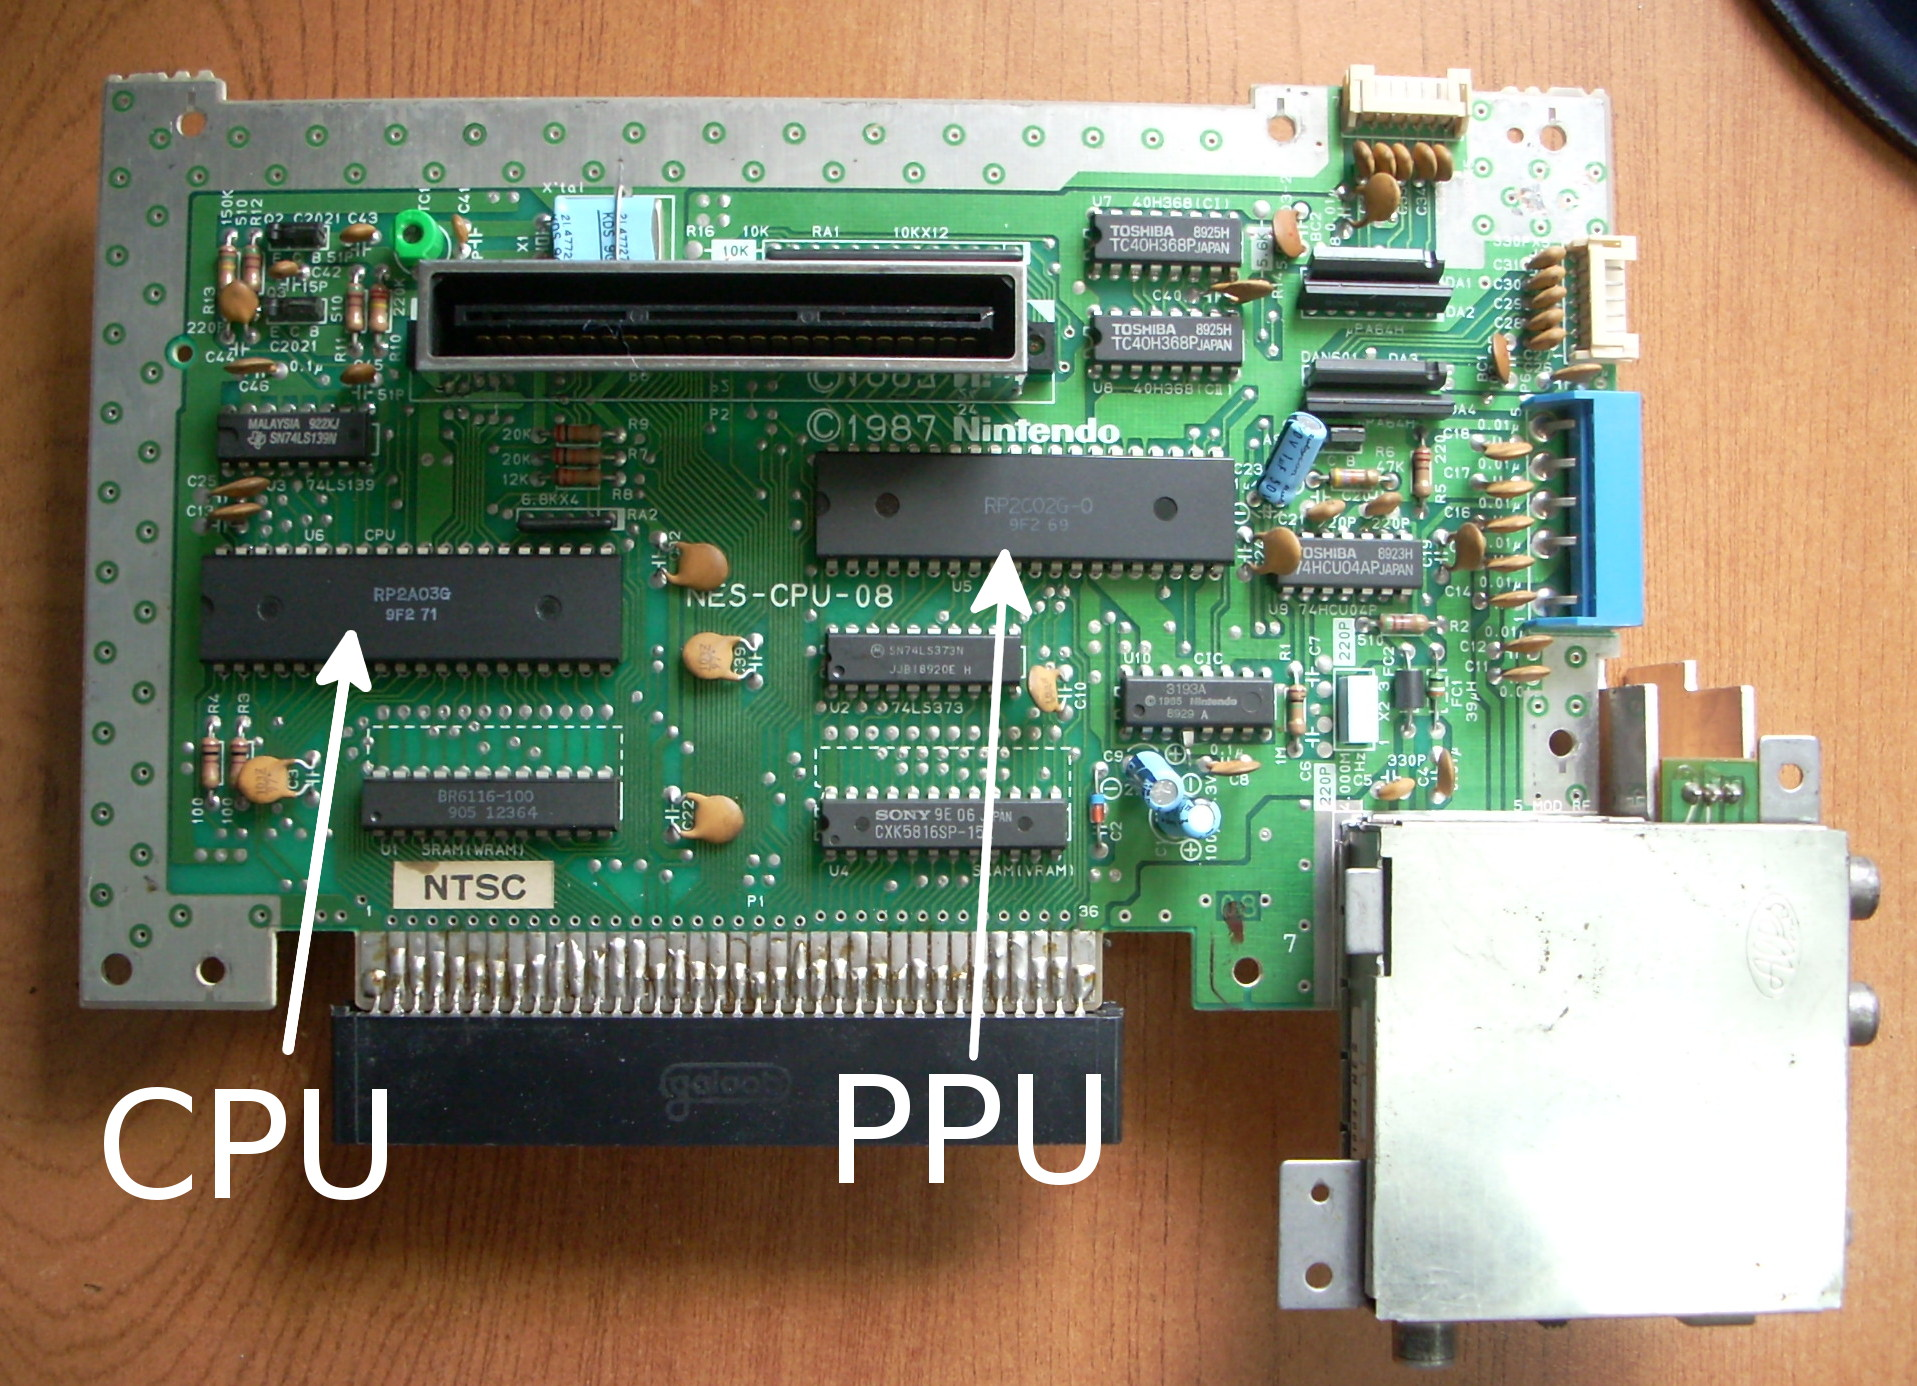
\includegraphics[width=0.6\textwidth]{hardware.jpg}
\end{wrapfigure}
La intención de que la consola sea más barata que la competencia de la época llevaron a que Nintento se decida a usar una Unidad de Procesamiento Central (CPU) desactualizada. Si bien un procesador de 16-bit hubiera sido lo óptimo, para mantener los precios bajos se decidieron a usar una variante del procesador 6502 de 8 bits, desarrolado por MOS techonology en 1975. El chip bastaría para ejecutar los programas, pero sería incapaz de generar los gráficos requeridos por lo que la compañía dicidió usar un segundo chip como una unidad totalmente dedicada al procesamiento de imagenes (Picture Processing Unit, PPU), responsable de calcular y mostrar los gráficos.



Ambos chips tienen su propia memoria interna, en forma de RAM. Los juegos son usualmente guardados en chips ROM\footnote{Read Only Memory} dentro del cartucho, el cual es accedido por la CPU cuando los mismos son insertados en el sistema.
La NES usa memory mapped I/O\footnote{Input/Output} para permitir al procesador comunicarse con sus otros componentes: la PPU y los dispositivos de entrada. La memory mapped I/O es una técnica donde la información puede ser transferida a un dispositivo mediante la escritura en una dirección espécifica en la memoria.


\section{CPU Memory Map}
\begin{figure}[H]\caption{Buses de la consola\label{fig:bus}}
\centering{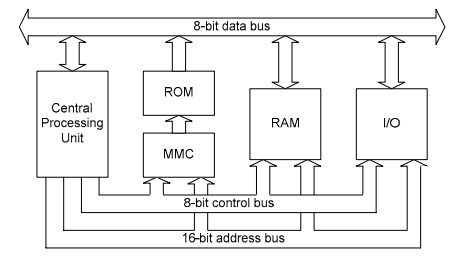
\includegraphics[width=0.8\textwidth]{bus.png}}
\end{figure}
La memoria está dividida en tres partes, la ROM dentro de los cartuchos, la RAM de la CPU y los registros I/O. El bus de direcciones es usado para establecer la dirección deseada. El bus de control es usado para informar a los componentes si el pedido es de lectura o escritura. El bus de datos es usado para leer o escribir el byte a la dirección elegida. Notemos que la ROM es de solo lectura y es accedida via el MMC, para permitir el cambio de bancos (explicado más abajo). Los registros I/O son usados para comunicarse con los otros componentes del sistema: la PPU y los dispositivos de entrada.

El chip 2A03 presente en la consola tiene un bus de direcciones de 16-bit y como tal puede soportar 64 KB de memoria en el rango \$0000-\$FFFF. La figura ~\ref{fig:memorymap} muestra el mapeo de memoria usado por la NES. El lado izquierdo es una versión simplificada mostrando las secciones más importantes, mientras que el lado derecho detalla cada sección.
\begin{figure}[H]\caption{Mapeo de la memoria\label{fig:memorymap}}
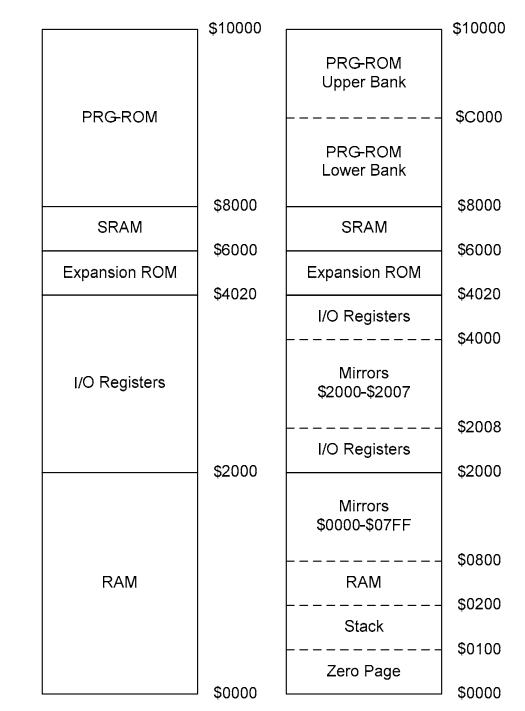
\includegraphics[width=0.8\textwidth]{memorymap.png}
\end{figure}


Zero Page se refiere a las direcciones en el rango \$0000-\$00FF, la primera página en memoria. La misma es usada por ciertos modos de acceso para lograr una ejecución más veloz. Las direcciones  \$0000-\$07FF están espejadas tres veces en \$0800-\$1FFF. Esto significa que por ejemplo, cualquier información escrita en \$0000 también se escribirá en \$0800, \$1000 y \$1800. Las direcciones \$2000-\$2007 están espejadas cada 8 bytes en la región \$2008-\$3FFF y los restantes registros siguen este espejado. SRAM (o WRAM) es la RAM de guardado, espacio usado para guardar las partidas.

A partir de \$8000 se encuentra la PRG-ROM\footnote{Program ROM} del cartucho. Juegos con solo un banco de 16 KB de PRG-ROM se cargaran tanto en \$8000 como en \$C000. Juegos con dos bancos de 16 KB de PRG-ROM, cargaran uno en \$8000 y otro en \$C000. Juegos con más de dos bancos usan mamory mappers para determinar que banco cargar en memoria. El memory mapper vigila las escrituras a una dirección específica (o rango de direcciones) y cuando esa dirección es escrita, realiza un cambio de bancos\footnote{Hace que la memoria mapee hacia un banco distinto al que se estaba usando}. Los detalles varían entre diferentes memory mappers. 

\section{Registros}
El 6502 tiene menos registros que procesadores similares. Existen tres registros especiales: el program counter, el stack pointer y el status register. También tiene tres registros generales: el acumulador y los registros X e Y, los cuales pueden ser usados para guardar o controlar información temporalmente.
\subsection{Program Counter (PC)}
\begin{itemize}
\item Program Counter (PC): Es un registro de 16 bits que guarda la dirección de la siguiente instrucción a ejecutar. El valor puede ser afectado por instrucciones de branch o jump, por llamadas e interrupciones.
\item Stack Pointer (SP): La pila esta ubicada en las direcciones \$0100-\$01FF. El stack pointer es un registro de 8 bits que sirve como un offset del \$0100. El stack crece de arriba hacia abajo, por lo que cuando un bits es insertado en el stack, el stack pointer es decrementado. No hay detección de stack overflow y el stack pointer pasara de \$00 a \$FF.

\item Acumulador (A): Es un registro de 8 bits que guarda los resultados de las operaciones aritméticas y lógicas. El acumulador también puede ser asignado a un valor cargado de memoria.

\item Registro X: El registro X es un registro de 8 bits tipicamente usado como contador o offset para algunos modos de acceso. El registro X puede ser asignado a un valor en memoria y puede ser usado para obtener o establecer el valor del stack pointer.

\item Registro Y: Es un registro de 8 bits, usado de la misma manera que el X, sólo que Y no puede afectar al stack pointer.

\item Processor Status (P): El registro de status contiene distintas flags de un bit cada una.
\begin{itemize}
\item Carry Flag (C): Se activa cuando la última instrucción resulta en un overflow del bit 7 o un underflow del bit 0.
\item Zero Flag (Z): Se activa si la última instrucción dio como resultado cero.
\item Interrupt Disable (I): Puede ser usado para evitar que el sistema responda a los IRQs. Es activado por la instrucción SEI (Set Interrupt Disable), las IRQs serán ignoradas hasta que se ejecute CLI (Clear Interrupt Disable).
\item Decimal Mode (D): Como el chip 2A03 no soporta el modo BCD, este flag es ignorado.
\item Break Command (B): Es usado para indicar que una instrucción BRK ha sido ejecutada, causando una IRQ.
\item Overflow Flag (V): Es activada si se obtuvo un resultado inválido en la instrucción anterior, tomando el complemento a dos del mismo.
\item Negative Flag (N): El bit 7 de un byte representa el signo de ese byte. Esta flag se activa si el bit de signo es 1.
\end{itemize}
Estos flags están dispuestos en el status register como muestra la figura ~\ref{fig:status}
\begin{figure}[H]\caption{Status Register\label{fig:status}}
\centering{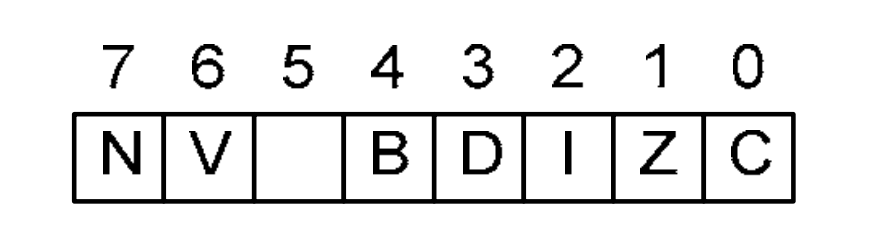
\includegraphics[width=0.5\textwidth]{status.png}}
\end{figure}
\end{itemize}

\section {Interrupciones}
Las interrupciones pueden ser generadas por software y por hardware. La NES tiene tres tipos diferentes que son NMI, IRQ y reset. Las direcciones a la cual saltar cuando una interrupción ocurre son guardadas en un arreglo (o vector table) en el PRG-ROM en \$FFFA-\$FFFF. Cuando una interrupción ocurre el sistema performa las siguientes acciones:
\begin{enumerate}
\item Reconocer el pedido de interrupción que ocurrió.
\item Completar la ejecución de la instrucción actual.
\item Poner el program counter y el status register en el stack
\item Activar el flag interrupt disable para prevenir interrupciones más adelante.
\item Cargar la dirección de la rutina encargada de procesar la interrupción desde la vector table al program counter.
\item Ejecutar la rutina correspondiente.
\item Luego de ejecutar la instrucción RTI (Return From Interrupt), obtener el program counter y el status desde el stack.
\item Continuar la ejecución del programa.
\end{enumerate}

Las \textbf{IRQs}, también llamadas maskable interrupt, son generadas por algunos memory mappers. Pueden ser iniciadas por software usando la instruccion BRK (Break). Cuando una IRQ ocurre el sistema salta a la dirección \$FFFE-\$FFFF.

La \textbf{NMI} (Non-Maskable Interrupt) es una interrupción generada por la PPU cuando la V-Blank ocurre al final de cada frame. NMI no es afectadas por el bit de interrupt disable. Sin embargo, NMI puede ser desactivada si el bit 7 del registro de control 1 del PPU (\$2000) es limpiado. Cuando una NMI ocurre el sistema salta a la dirección localizada en \$FFFA-\$FFFB.

La interrupción reset es iniciada al comienzo del sistema y cuando el usuario presiona el botón de reinicio. Cuando esta ocurre el sistema salta a la dirección \$FFFC-\$FFFD.

El sistema da mayor prioridad a las interrupción reset, seguida de NMI y finalmente IRQ.
La consola tiene una latencia de interrupción de 7 ciclos, que implica que tarda 7 ciclos del CPU para comenzar a ejecutar la rutina de interrupción.


\section{Modos de Acceso}
El 6502 tiene distintos modos de acceso, los cuales proveen distintas formas de acceder a memoria. Hay algunos que operan sobre los contenidos de registros. En total existen 13 modos distintos. Los mismos se detallan en \cite[p.~39]{nesdoc}
\section{Instrucciones}

El procesador tiene 56 instrucciones diferentes aunque algunas se repiten, usando distintos modos de acceso haciendo un total de 151 opcodes válidos de un posible total de 256. Las instrucciones tienen uno, dos o tres bytes de longitud, dependiendo del modo de acceso. El primer byte es el opcode y los restantes los operandos.

\subsection{Implementación}

Para sintetizar todas las instrucciones necesarias en el código, se descompuso cada instrucción en micro-operaciones. Por ejemplo para hacer un ADD (suma), primero se traen los operandos de memoria o de registros, luego se efectua la suma, después se guarda el resultado en el registro correspondiente y por último se modifican las flags del status register adecuadas. Cada uno de estos pasos es una micro-operación.

Se puede aprovechar el hecho de que sólo se necesitan 56 micro-operaciones para poder expresar \emph{todas} las instrucciones del procesador, para lograr un emulador del procesador mucho más corto en terminos de código.

El procedimiento que se siguió fue el siguiente. Se juntaron todas las micro-operaciones en una misma función, que recibe la instrucción a ejecutar. Para cada micro-instrucción se decide si se debe ejecutar o no, usando una máscara de 256 bits (un bit por cada instrucción). Así, si el bit i de la máscara correspondiente a la micro-instrucción j es 1, significa que j es una de las micro-instrucciones que componen la instrucción i.
En otras palabras, para cada operación se accede a las máscaras de bits de cada una de las micro-instrucciones y si el bit resulta uno la micro-operación es ejecutada.

Para evitar acceder a la máscara de bits en tiempo de ejecución, se usaron templates (C++) las cuales realizan todo el proceso de las máscaras de bits en tiempo de compilación, lo que lleva a un ejecutable con 256 funciones (una para cada operación) automáticamente sintetizadas.

Para guardar las máscaras de bits en el código, se utilizó una codificación especial, la cual está detallada en util/specs/base256-explained.txt .


\section{PPU}
No se pretende explicar en detalle el completo funcionamiento de la parte gráfica de la consola. La PPU tiene una memoria separada de la CPU con su propio memory map, y a su vez contiene cuatro registros que controlan mediante distintos bits su funcionamiento. Para información detallada puede consultar \cite[p.~16]{nesdoc} y los documentos disponibles en \cite{techdocs}.

\subsection{Colores}
La consola cuenta con 52 colores. Pero no todos pueden usarse a la vez. Existen dos paletas de 16 colores, la paleta de imagen y la de sprites, en cada una no se guardan los colores, sino los índices a los colores del sistema.

\subsection{Composición de la pantalla}
Cada frame que es mostrado en la pantalla está formado por el fondo y los sprites (objetos móviles). El fondo en un principio estaría fijo, pero es posible configurar la PPU para que el fondo se vaya desplazando horizontal por ejemplo, tal como lo hacía Super Mario Bros. Tanto los sprites como el fondo se dividen en 'tiles' de 8x8 pixeles, todos estos tiles son guardados en la pattern table, ubicada en la memoria PPU. Para saber que tile va en que lugar de la pantalla se usan los name tables. Cada name table está asociada a un pattern table. No se pretende ahondar en el tema, pero combinando la información del tile con la pattern table se obtiene el color del pixel resultante.

\subsection{Proceso de dibujado}

Las imagenes son mostradas en la televisión por un rayo de electrones a alta velocidad que se mueve por la pantalla, de izquierda a derecha, dibujando cada pixel. Una sóla lina de pixeles es llamada scanline. Al final de cada scanline el rayo de electrones debe moverse a la siguiente línea y retornar a la izquierda antes de proceder. El tiempo que tarda en hacer esto es conocido como periodo Horizontal Blank (H-Blank).

Luego de dibujar la pantalla una vez, el rayo de electrones debe retornar a la izquina superior izquierda, para empezar el siguiente frame. El tiempo que toma hacer esto es conocido como el periodo Vertical Blank (V-Blank). Cuando el periodo V-Blank comienza, la PPU prende el bit 7 del registro I/O \$2002.

Para ver el proceso completo realizado por el emulador ver el archivo emulador/ppu.cpp, línea 249.



